\documentclass[14pt,a4paper]{extarticle}\usepackage[]{graphicx}\usepackage[]{xcolor}
% maxwidth is the original width if it is less than linewidth
% otherwise use linewidth (to make sure the graphics do not exceed the margin)
\makeatletter
\def\maxwidth{ %
  \ifdim\Gin@nat@width>\linewidth
    \linewidth
  \else
    \Gin@nat@width
  \fi
}
\makeatother

\definecolor{fgcolor}{rgb}{0.345, 0.345, 0.345}
\newcommand{\hlnum}[1]{\textcolor[rgb]{0.686,0.059,0.569}{#1}}%
\newcommand{\hlsng}[1]{\textcolor[rgb]{0.192,0.494,0.8}{#1}}%
\newcommand{\hlcom}[1]{\textcolor[rgb]{0.678,0.584,0.686}{\textit{#1}}}%
\newcommand{\hlopt}[1]{\textcolor[rgb]{0,0,0}{#1}}%
\newcommand{\hldef}[1]{\textcolor[rgb]{0.345,0.345,0.345}{#1}}%
\newcommand{\hlkwa}[1]{\textcolor[rgb]{0.161,0.373,0.58}{\textbf{#1}}}%
\newcommand{\hlkwb}[1]{\textcolor[rgb]{0.69,0.353,0.396}{#1}}%
\newcommand{\hlkwc}[1]{\textcolor[rgb]{0.333,0.667,0.333}{#1}}%
\newcommand{\hlkwd}[1]{\textcolor[rgb]{0.737,0.353,0.396}{\textbf{#1}}}%
\let\hlipl\hlkwb

\usepackage{framed}
\makeatletter
\newenvironment{kframe}{%
 \def\at@end@of@kframe{}%
 \ifinner\ifhmode%
  \def\at@end@of@kframe{\end{minipage}}%
  \begin{minipage}{\columnwidth}%
 \fi\fi%
 \def\FrameCommand##1{\hskip\@totalleftmargin \hskip-\fboxsep
 \colorbox{shadecolor}{##1}\hskip-\fboxsep
     % There is no \\@totalrightmargin, so:
     \hskip-\linewidth \hskip-\@totalleftmargin \hskip\columnwidth}%
 \MakeFramed {\advance\hsize-\width
   \@totalleftmargin\z@ \linewidth\hsize
   \@setminipage}}%
 {\par\unskip\endMakeFramed%
 \at@end@of@kframe}
\makeatother

\definecolor{shadecolor}{rgb}{.97, .97, .97}
\definecolor{messagecolor}{rgb}{0, 0, 0}
\definecolor{warningcolor}{rgb}{1, 0, 1}
\definecolor{errorcolor}{rgb}{1, 0, 0}
\newenvironment{knitrout}{}{} % an empty environment to be redefined in TeX

\usepackage{alltt}

\usepackage{fontspec}
\setmainfont{Times New Roman}
\usepackage{geometry}
\geometry{margin=2.5cm}
\usepackage{graphicx}
\usepackage{amsmath}
\usepackage{booktabs}
\usepackage{microtype}
\usepackage[colorlinks=true, linkcolor=blue, urlcolor=blue, citecolor=blue]{hyperref}

% Tiếng Việt không có luật ngắt từ trong LaTeX; cho phép giãn nhẹ khoảng
% cách để tránh chữ tràn ra lề (thay vì để dòng bị overfull).
\tolerance=2000
\emergencystretch=3em

\title{Xây dựng mô hình dự đoán bệnh gan trên dữ liệu ILPD:\\
Ứng dụng Bootstrap và K-fold Cross-Validation}
\author{Nguyen Ho Bao Thien}
\date{\today}
\IfFileExists{upquote.sty}{\usepackage{upquote}}{}
\begin{document}

\maketitle
\tableofcontents
\newpage



\section{Đặt vấn đề}

% Viết ở đây: bài toán Data Science đầy đủ - xây dựng mô hình dự đoán bệnh
% gan từ chỉ số sinh hóa (bài toán phân loại nhị phân). Nhưng thay vì chỉ
% báo cáo 1 con số accuracy, tiểu luận này đi sâu vào 2 câu hỏi:
%   1) Trong các mô hình có thể xây, mô hình nào thực sự dự đoán tốt nhất
%      trên dữ liệu MỚI (chưa thấy)? -> cần K-fold CV để chọn & tinh chỉnh
%      mô hình một cách khách quan, tránh overfitting khi so sánh.
%   2) Mô hình cuối cùng được chọn có đáng tin cậy không - hiệu năng của nó
%      ổn định hay dao động mạnh, các hệ số có thực sự quan trọng hay chỉ
%      do may rủi của mẫu? -> cần Bootstrap để ước lượng CI cho hiệu năng
%      và độ ổn định của mô hình.
% Nói cách khác: K-fold giúp CHỌN mô hình đúng đắn, Bootstrap giúp TRẢ LỜI
% mô hình đó có đáng tin hay không.

\section{Cơ sở lý thuyết}

Hai phương pháp được trình bày trong chương này --- Bootstrap và K-fold
Cross-Validation --- đều thuộc nhóm kỹ thuật \emph{resampling} (lấy mẫu
lại) và cùng xuất phát từ một khó khăn nền tảng của thống kê ứng dụng:
nhà nghiên cứu chỉ quan sát được \emph{một} mẫu hữu hạn rút ra từ tổng
thể, trong khi mọi đại lượng tính từ mẫu đó --- giá trị trung bình, hệ số
hồi quy, hay độ chính xác của một mô hình --- đều là biến ngẫu nhiên và
sẽ nhận giá trị khác đi nếu ta rút được một mẫu khác. Câu hỏi cốt lõi vì
thế không dừng ở ``giá trị ước lượng bằng bao nhiêu'' mà là ``ước lượng
đó dao động đến mức nào và có thể tin cậy tới đâu''. Khi công thức lý
thuyết cho phân phối lấy mẫu không tồn tại hoặc quá phức tạp, các phương
pháp resampling cho phép \emph{mô phỏng} lại chính sự biến thiên đó từ dữ
liệu sẵn có, bằng cách sinh ra nhiều mẫu con và quan sát đại lượng quan
tâm thay đổi ra sao qua các mẫu con ấy.

\subsection{Phương pháp Bootstrap}

Bootstrap là phương pháp resampling do Bradley Efron giới thiệu năm 1979,
dùng để ước lượng độ chính xác --- sai số chuẩn, độ chệch, khoảng tin cậy
--- của một đại lượng thống kê mà không cần giả định về dạng phân phối của
tổng thể và không cần thu thập thêm dữ liệu.

\textbf{Nền tảng lý thuyết.} Giả sử ta quan tâm tới một tham số tổng thể
$\theta = \theta(F)$, trong đó $F$ là hàm phân phối chưa biết của tổng
thể; từ mẫu quan sát $x_1, \ldots, x_n$ ta tính được ước lượng
$\hat{\theta} = \theta(\hat{F})$. Để đánh giá độ chính xác của
$\hat{\theta}$, về mặt lý tưởng ta cần biết \emph{phân phối lấy mẫu}
(sampling distribution) của nó --- tức tập hợp các giá trị mà
$\hat{\theta}$ có thể nhận nếu quá trình rút mẫu kích thước $n$ từ $F$
được lặp lại vô số lần. Trong thực tế điều này bất khả thi, bởi $F$ không
biết và ta chỉ có duy nhất một mẫu. Ý tưởng then chốt của Efron là thay
tổng thể chưa biết $F$ bằng \emph{phân phối thực nghiệm} $\hat{F}$ ---
phân phối rời rạc gán xác suất $1/n$ cho mỗi quan sát đã có. Theo định lý
Glivenko--Cantelli, $\hat{F}$ hội tụ đều về $F$ khi cỡ mẫu tăng, nên với
$n$ đủ lớn $\hat{F}$ là một thay thế hợp lý cho $F$. Việc rút một mẫu kích
thước $n$ từ $\hat{F}$ chính là lấy mẫu ngẫu nhiên \textbf{có hoàn lại} từ
dữ liệu gốc. Đây là nội dung của \emph{nguyên lý plug-in}: phân phối lấy
mẫu của $\hat{\theta}$ dưới $F$ được xấp xỉ bằng phân phối của các ước
lượng bootstrap $\hat{\theta}^{*}$ tính dưới $\hat{F}$.

\textbf{Thuật toán.}
\begin{enumerate}
  \item Từ mẫu gốc kích thước $n$, lấy mẫu ngẫu nhiên \textbf{có hoàn lại}
        kích thước $n$, gọi là mẫu bootstrap thứ $b$.
  \item Tính thống kê quan tâm $\hat{\theta}^{*}_{b}$ (trung bình, trung
        vị, hệ số hồi quy, AUC, \ldots) trên mẫu bootstrap này.
  \item Lặp lại bước 1--2 $B$ lần ($B$ thường từ 500 đến vài nghìn), thu
        được $\hat{\theta}^{*}_{1}, \ldots, \hat{\theta}^{*}_{B}$.
  \item Dùng phân phối thực nghiệm của $B$ giá trị này để ước lượng sai số
        chuẩn và khoảng tin cậy của $\hat{\theta}$.
\end{enumerate}

\textbf{Ước lượng sai số chuẩn và khoảng tin cậy.} Sai số chuẩn bootstrap
được ước lượng bằng độ lệch chuẩn của $B$ giá trị thống kê:
\[
  \widehat{SE}_{boot} = \sqrt{\frac{1}{B-1}\sum_{b=1}^{B}
  \left(\hat{\theta}^{*}_{b} - \bar{\theta}^{*}\right)^2}, \qquad
  \bar{\theta}^{*} = \frac{1}{B}\sum_{b=1}^{B}\hat{\theta}^{*}_{b}.
\]
Khoảng tin cậy theo \emph{phương pháp phân vị} (percentile) ở mức tin cậy
$1-\alpha$ là $\big[\hat{\theta}^{*}_{(\alpha/2)},\,
\hat{\theta}^{*}_{(1-\alpha/2)}\big]$, với $\hat{\theta}^{*}_{(q)}$ là
phân vị mức $q$ của tập $B$ giá trị bootstrap; chẳng hạn ở mức 95\% ta lấy
phân vị 2,5\% và 97,5\%. Một cách tinh vi hơn là \emph{BCa
(bias-corrected and accelerated)}, hiệu chỉnh thêm độ chệch và độ xiên
của phân phối bootstrap để cho khoảng tin cậy chính xác hơn khi phân phối
không đối xứng.

\textbf{Ví dụ minh hoạ.} Giả sử ta muốn ước lượng khoảng tin cậy cho
\emph{trung vị} nồng độ Total Bilirubin ở nhóm bệnh nhân mắc bệnh gan.
Trung vị không có công thức sai số chuẩn đơn giản như trung bình, nên đây
là tình huống điển hình để dùng bootstrap. Ta rút $B = 1000$ mẫu có hoàn
lại từ tập giá trị Total Bilirubin gốc; mỗi mẫu cho một trung vị
$\hat{\theta}^{*}_{b}$. Độ lệch chuẩn của 1000 trung vị này là ước lượng
sai số chuẩn, còn khoảng giữa phân vị 2,5\% và 97,5\% của chúng cho ta
khoảng tin cậy 95\% cho trung vị tổng thể. Thực nghiệm cụ thể trên dữ liệu
ILPD được trình bày ở phần thực hành.

\textbf{Một biến thể phổ biến: .632 bootstrap.} Trong mỗi mẫu bootstrap
kích thước $n$, xác suất một quan sát cụ thể không được chọn ở một lần rút
là $1 - 1/n$; sau $n$ lần rút, xác suất nó hoàn toàn vắng mặt là
$(1 - 1/n)^{n} \to e^{-1} \approx 0{,}368$. Do đó trung bình mỗi mẫu
bootstrap chỉ chứa khoảng 63,2\% số quan sát khác nhau, còn 36,8\% quan
sát còn lại (\emph{out-of-bag}, OOB) không tham gia huấn luyện và có thể
dùng làm tập kiểm tra độc lập. Biến thể \textbf{.632 bootstrap} khai thác
tính chất này để ước lượng sai số dự đoán của mô hình, bằng cách kết hợp
sai số huấn luyện (thường quá lạc quan) với sai số trên phần out-of-bag
theo trọng số cố định:
\[
  \widehat{Err}_{.632} = 0{,}368 \cdot \overline{err}
  + 0{,}632 \cdot \widehat{Err}_{OOB},
\]
trong đó $\overline{err}$ là sai số trên tập huấn luyện và
$\widehat{Err}_{OOB}$ là sai số trung bình trên các quan sát OOB; trọng
số $0{,}632$ phản ánh đúng tỉ lệ quan sát trung bình có mặt trong
mẫu bootstrap. Phiên bản cải tiến \emph{.632+} còn điều chỉnh trọng số này
theo mức độ overfitting của mô hình. Đây chính là phương pháp được dùng ở
phần thực hành để đối chiếu với kết quả K-fold Cross-Validation.

\textbf{Ưu điểm.} Không đòi hỏi giả định về phân phối tổng thể; áp dụng
được cho hầu như mọi thống kê, kể cả những thống kê không có công thức sai
số chuẩn lý thuyết (trung vị, hệ số trong mô hình phi tuyến, AUC, \ldots).

\textbf{Nhược điểm.} Tốn chi phí tính toán do phải lặp lại hàng trăm đến
hàng nghìn lần; có thể cho kết quả chệch với cỡ mẫu nhỏ; đồng thời giả
định ngầm rằng dữ liệu độc lập và cùng phân phối (i.i.d.), nên không áp
dụng trực tiếp được cho dữ liệu có cấu trúc phụ thuộc như chuỗi thời gian
(khi đó cần dùng biến thể \emph{block bootstrap}).

\subsection{Phương pháp K-fold Cross-Validation}

K-fold Cross-Validation (kiểm định chéo $k$ phần) là kỹ thuật resampling
\textbf{không hoàn lại}, dùng để ước lượng sai số dự đoán của một mô hình
trên dữ liệu chưa từng thấy (generalization error), qua đó tránh việc
đánh giá mô hình ngay trên chính dữ liệu đã dùng để huấn luyện nó.

\textbf{Nền tảng lý thuyết.} Khi xây dựng một mô hình dự đoán, mục tiêu
không phải là mô tả thật khớp dữ liệu đã có mà là dự đoán chính xác trên
dữ liệu \emph{mới}. Nếu đánh giá mô hình ngay trên dữ liệu huấn luyện, ta
sẽ thu được ước lượng quá lạc quan, bởi mô hình đã ``học thuộc'' cả những
dao động ngẫu nhiên riêng của mẫu --- hiện tượng \emph{overfitting}. Cách
khắc phục đơn giản nhất là tách riêng một phần dữ liệu làm tập kiểm tra
(holdout), nhưng cách này vừa lãng phí dữ liệu, vừa cho kết quả phụ thuộc
mạnh vào một lần chia ngẫu nhiên duy nhất, khiến ước lượng có phương sai
lớn khi mẫu nhỏ. K-fold Cross-Validation khắc phục đồng thời cả hai hạn
chế bằng cách luân phiên vai trò huấn luyện/kiểm tra qua $k$ lần chia, sao
cho mọi quan sát đều được dùng để kiểm tra đúng một lần và dùng để huấn
luyện $k-1$ lần.

\textbf{Thuật toán.}
\begin{enumerate}
  \item Chia ngẫu nhiên dữ liệu thành $k$ phần (fold) rời nhau, kích
        thước xấp xỉ bằng nhau.
  \item Với mỗi $i = 1, \ldots, k$: dùng $k-1$ phần còn lại để huấn luyện
        mô hình, phần thứ $i$ dùng để kiểm tra.
  \item Tính sai số dự đoán trên từng fold, sau đó lấy trung bình:
\[
  CV_{(k)} = \frac{1}{k}\sum_{i=1}^{k}
  L\!\left(y_i,\, \hat{f}^{(-i)}(x_i)\right),
\]
        với $L$ là hàm mất mát (tỉ lệ phân loại sai, MSE, \ldots) và
        $\hat{f}^{(-i)}$ là mô hình được huấn luyện mà không dùng fold thứ
        $i$.
\end{enumerate}

\textbf{Ví dụ minh hoạ.} Xét bài toán phân loại bệnh gan trên ILPD với
$n = 579$ quan sát (sau khi loại các dòng khuyết) và mô hình hồi quy
logistic. Với $k = 10$, dữ liệu được chia thành 10 phần, mỗi phần khoảng
58 quan sát. Ở lần lặp thứ nhất, 9 phần (khoảng 521 quan sát) được dùng để
ước lượng các hệ số của mô hình, phần còn lại dùng để dự đoán và tính sai
số phân loại; quá trình lặp lại 10 lần, mỗi phần lần lượt đóng vai tập
kiểm tra. Trung bình 10 sai số này là ước lượng sai số dự đoán của mô
hình, còn độ lệch chuẩn giữa chúng phản ánh mức độ ổn định của mô hình qua
các cách chia dữ liệu khác nhau.

\textbf{Một biến thể phổ biến: Stratified k-fold.} Khi biến mục tiêu mất
cân bằng lớp, việc chia fold hoàn toàn ngẫu nhiên có thể tạo ra những fold
có tỉ lệ lớp lệch hẳn so với tổng thể, thậm chí thiếu vắng lớp thiểu số,
làm cho ước lượng sai số bị nhiễu. \textbf{Stratified k-fold} (kiểm định
chéo phân tầng) khắc phục bằng cách chia sao cho \emph{mỗi fold giữ nguyên
tỉ lệ các lớp} như trong toàn bộ dữ liệu. Với ILPD --- nơi tỉ lệ giữa
nhóm mắc bệnh và không mắc bệnh xấp xỉ 71\%/29\% --- mỗi fold trong số 10
fold được ràng buộc để duy trì đúng tỉ lệ đó, nhờ vậy mỗi lần kiểm tra đều
phản ánh đúng cơ cấu lớp thực tế và cho ước lượng ổn định hơn. Đây cũng là
lựa chọn mặc định của hàm \texttt{trainControl} trong gói \texttt{caret}
khi biến mục tiêu là biến phân loại, và được áp dụng trong toàn bộ phần
thực hành. Ngoài ra còn hai biến thể đáng chú ý khác: \emph{Leave-One-Out
CV} (trường hợp đặc biệt khi $k = n$) và \emph{Repeated k-fold} (lặp lại
toàn bộ quy trình nhiều lần với các cách chia khác nhau để giảm thêm
phương sai của ước lượng).

\textbf{Vai trò trong quy trình Data Science.} K-fold CV không chỉ dùng để
\emph{đánh giá} một mô hình đơn lẻ, mà còn là công cụ khách quan để
\emph{so sánh nhiều mô hình} với nhau và \emph{tinh chỉnh siêu tham số}
(hyperparameter tuning, chẳng hạn chọn \texttt{mtry} cho Random Forest hay
\texttt{cp} cho Decision Tree). Điều kiện tiên quyết là việc tinh chỉnh
phải được thực hiện hoàn toàn bên trong vòng lặp CV, nhằm tránh hiện tượng
``nhìn trộm'' tập kiểm tra (data leakage) khi lựa chọn mô hình.

\textbf{Ưu điểm.} Mọi quan sát đều được dùng để kiểm tra đúng một lần nên
ước lượng sai số ít lạc quan hơn so với chỉ chia train/test một lần; áp
dụng được cho bất kỳ thuật toán học máy nào.

\textbf{Nhược điểm.} Chi phí tính toán tăng tuyến tính theo $k$ (hoặc theo
$n$ với LOOCV); kết quả có thể có phương sai cao khi $k$ nhỏ, vì mỗi lần
chỉ ước lượng trên một phần nhỏ dữ liệu.

\subsection{So sánh và vai trò bổ sung của hai phương pháp trong quy trình Data Science}

Hai phương pháp có chung bản chất resampling nhưng phục vụ hai mục tiêu
khác nhau và đánh đổi bias--variance theo hai hướng ngược nhau:

\begin{center}
\small
\begin{tabular}{@{}p{2.6cm}p{5.9cm}p{5.9cm}@{}}
\toprule
 & \textbf{Bootstrap} & \textbf{K-fold CV} \\
\midrule
Cách lấy mẫu & Có hoàn lại & Không hoàn lại \\
Mục tiêu chính & Ước lượng độ tin cậy (SE, CI) của một thống kê & Ước lượng sai số dự đoán, chọn/so sánh mô hình \\
Xu hướng bias & Có thể lạc quan nếu không hiệu chỉnh (.632+) & Xấp xỉ không chệch với sai số dự đoán thật \\
Xu hướng variance & Thấp hơn (nhiều mẫu, chồng lấp nhiều) & Cao hơn khi $k$ nhỏ (mỗi fold độc lập hơn) \\
Chi phí tính toán & Cao (B thường 500--2000 lần lặp) & Vừa phải ($k$ thường 5--10 lần lặp) \\
\bottomrule
\end{tabular}
\end{center}

Nói cách khác: \textbf{K-fold CV giúp CHỌN mô hình đúng đắn} (dựa trên ước
lượng khách quan về khả năng tổng quát hoá), còn \textbf{Bootstrap giúp
TRẢ LỜI mô hình đã chọn đó có đáng tin cậy hay không} (thông qua khoảng
tin cậy cho hiệu năng và cho từng hệ số của mô hình). Đây chính là trình
tự được áp dụng trong các phần thực hành tiếp theo của tiểu luận: dữ liệu
được tiền xử lý, sau đó K-fold CV được dùng để so sánh và chọn ra mô hình
tốt nhất, và cuối cùng Bootstrap được dùng để đánh giá độ tin cậy của
chính mô hình đó.

\section{Dữ liệu và tiền xử lý}

Bộ dữ liệu \textbf{ILPD (Indian Liver Patient Dataset)} gồm 583 quan sát,
10 biến đặc trưng (sinh hóa + nhân khẩu học) và 1 biến mục tiêu
(\texttt{Selector}: mắc bệnh gan hay không). Chi tiết mô tả biến xem tại
\texttt{README.md} của dự án.

\begin{knitrout}\scriptsize
\definecolor{shadecolor}{rgb}{0.969, 0.969, 0.969}\color{fgcolor}\begin{kframe}
\begin{alltt}
\hlkwd{library}\hldef{(boot)}
\hlkwd{library}\hldef{(caret)}
\hlkwd{library}\hldef{(pROC)}
\hlkwd{library}\hldef{(dplyr)}
\hlkwd{library}\hldef{(ggplot2)}
\hlkwd{library}\hldef{(randomForest)}
\hlkwd{library}\hldef{(rpart)}

\hlkwd{set.seed}\hldef{(}\hlnum{2024}\hldef{)}
\end{alltt}
\end{kframe}
\end{knitrout}

\begin{knitrout}\scriptsize
\definecolor{shadecolor}{rgb}{0.969, 0.969, 0.969}\color{fgcolor}\begin{kframe}
\begin{alltt}
\hldef{df} \hlkwb{<-} \hlkwd{read.csv}\hldef{(}\hlsng{"Indian Liver Patient Dataset (ILPD).csv"}\hldef{,} \hlkwc{header} \hldef{=} \hlnum{FALSE}\hldef{)}
\hlkwd{colnames}\hldef{(df)} \hlkwb{<-} \hlkwd{c}\hldef{(}\hlsng{"Age"}\hldef{,} \hlsng{"Gender"}\hldef{,} \hlsng{"TB"}\hldef{,} \hlsng{"DB"}\hldef{,} \hlsng{"Alkphos"}\hldef{,} \hlsng{"Sgpt"}\hldef{,} \hlsng{"Sgot"}\hldef{,}
                   \hlsng{"TP"}\hldef{,} \hlsng{"ALB"}\hldef{,} \hlsng{"AG_Ratio"}\hldef{,} \hlsng{"Selector"}\hldef{)}

\hldef{df}\hlopt{$}\hldef{Selector} \hlkwb{<-} \hlkwd{factor}\hldef{(df}\hlopt{$}\hldef{Selector,} \hlkwc{levels} \hldef{=} \hlkwd{c}\hldef{(}\hlnum{1}\hldef{,} \hlnum{2}\hldef{),}
                       \hlkwc{labels} \hldef{=} \hlkwd{c}\hldef{(}\hlsng{"Disease"}\hldef{,} \hlsng{"NoDisease"}\hldef{))}
\hldef{df}\hlopt{$}\hldef{Gender}   \hlkwb{<-} \hlkwd{factor}\hldef{(df}\hlopt{$}\hldef{Gender)}

\hlkwd{sum}\hldef{(}\hlkwd{is.na}\hldef{(df))}
\end{alltt}
\begin{verbatim}
## [1] 4
\end{verbatim}
\begin{alltt}
\hldef{df} \hlkwb{<-} \hlkwd{na.omit}\hldef{(df)}

\hlkwd{table}\hldef{(df}\hlopt{$}\hldef{Selector)}
\end{alltt}
\begin{verbatim}
## 
##   Disease NoDisease 
##       414       165
\end{verbatim}
\begin{alltt}
\hlkwd{prop.table}\hldef{(}\hlkwd{table}\hldef{(df}\hlopt{$}\hldef{Selector))}
\end{alltt}
\begin{verbatim}
## 
##   Disease NoDisease 
## 0.7150259 0.2849741
\end{verbatim}
\end{kframe}
\end{knitrout}

% Viết ở đây: nhận xét về mất cân bằng lớp (~71% Disease / 29% NoDisease),
% vì sao điều này quan trọng khi chọn k-fold (nên dùng stratified k-fold,
% caret::trainControl mặc định đã stratify theo biến outcome).

\subsection{Khám phá dữ liệu (EDA)}

\begin{knitrout}\scriptsize
\definecolor{shadecolor}{rgb}{0.969, 0.969, 0.969}\color{fgcolor}\begin{kframe}
\begin{alltt}
\hlkwd{summary}\hldef{(df)}
\end{alltt}
\begin{verbatim}
##       Age           Gender          TB               DB        
##  Min.   : 4.00   Female:140   Min.   : 0.400   Min.   : 0.100  
##  1st Qu.:33.00   Male  :439   1st Qu.: 0.800   1st Qu.: 0.200  
##  Median :45.00                Median : 1.000   Median : 0.300  
##  Mean   :44.78                Mean   : 3.315   Mean   : 1.494  
##  3rd Qu.:58.00                3rd Qu.: 2.600   3rd Qu.: 1.300  
##  Max.   :90.00                Max.   :75.000   Max.   :19.700  
##     Alkphos            Sgpt              Sgot              TP       
##  Min.   :  63.0   Min.   :  10.00   Min.   :  10.0   Min.   :2.700  
##  1st Qu.: 175.5   1st Qu.:  23.00   1st Qu.:  25.0   1st Qu.:5.800  
##  Median : 208.0   Median :  35.00   Median :  42.0   Median :6.600  
##  Mean   : 291.4   Mean   :  81.13   Mean   : 110.4   Mean   :6.482  
##  3rd Qu.: 298.0   3rd Qu.:  61.00   3rd Qu.:  87.0   3rd Qu.:7.200  
##  Max.   :2110.0   Max.   :2000.00   Max.   :4929.0   Max.   :9.600  
##       ALB           AG_Ratio           Selector  
##  Min.   :0.900   Min.   :0.3000   Disease  :414  
##  1st Qu.:2.600   1st Qu.:0.7000   NoDisease:165  
##  Median :3.100   Median :0.9300                  
##  Mean   :3.139   Mean   :0.9471                  
##  3rd Qu.:3.800   3rd Qu.:1.1000                  
##  Max.   :5.500   Max.   :2.8000
\end{verbatim}
\begin{alltt}
\hlkwd{ggplot}\hldef{(df,} \hlkwd{aes}\hldef{(}\hlkwc{x} \hldef{= Selector,} \hlkwc{y} \hldef{= TB,} \hlkwc{fill} \hldef{= Selector))} \hlopt{+}
  \hlkwd{geom_boxplot}\hldef{()} \hlopt{+}
  \hlkwd{labs}\hldef{(}\hlkwc{title} \hldef{=} \hlsng{"Phân phối Total Bilirubin (TB) theo nhóm bệnh"}\hldef{,} \hlkwc{y} \hldef{=} \hlsng{"TB"}\hldef{,} \hlkwc{x} \hldef{=} \hlkwa{NULL}\hldef{)}
\end{alltt}
\end{kframe}\begin{figure}

{\centering 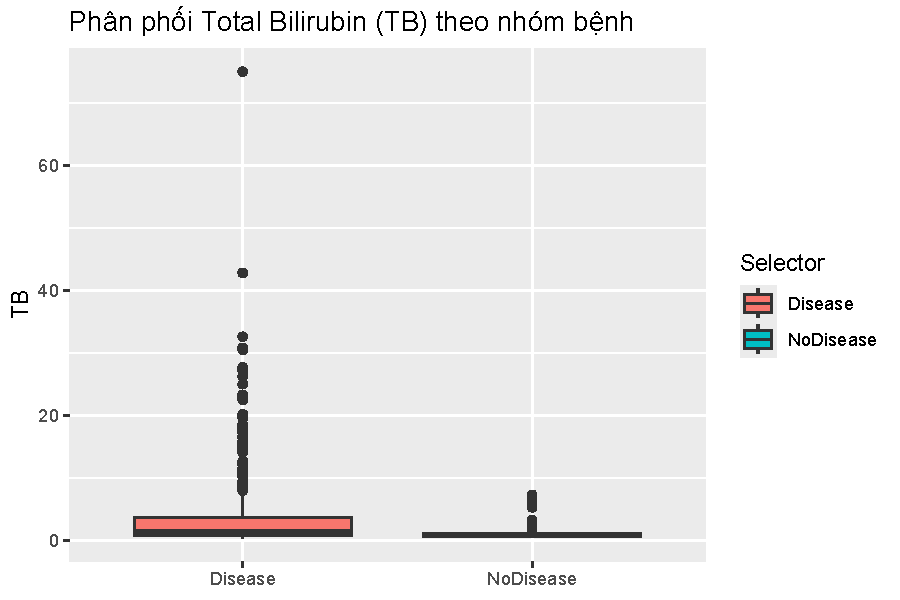
\includegraphics[width=\maxwidth]{figure/eda-1} 

}

\caption[Phân phối Total Bilirubin (TB) theo nhóm bệnh]{Phân phối Total Bilirubin (TB) theo nhóm bệnh}\label{fig:eda}
\end{figure}

\end{knitrout}

\begin{knitrout}\scriptsize
\definecolor{shadecolor}{rgb}{0.969, 0.969, 0.969}\color{fgcolor}\begin{kframe}
\begin{alltt}
\hlcom{# Các enzyme gan (Sgpt, Sgot, Alkphos) thường lệch phải rất mạnh}
\hlkwd{ggplot}\hldef{(df,} \hlkwd{aes}\hldef{(}\hlkwc{x} \hldef{= Sgpt))} \hlopt{+}
  \hlkwd{geom_histogram}\hldef{(}\hlkwc{bins} \hldef{=} \hlnum{40}\hldef{)} \hlopt{+}
  \hlkwd{labs}\hldef{(}\hlkwc{title} \hldef{=} \hlsng{"Phân phối Sgpt (trước khi biến đổi log)"}\hldef{)}
\end{alltt}
\end{kframe}\begin{figure}

{\centering 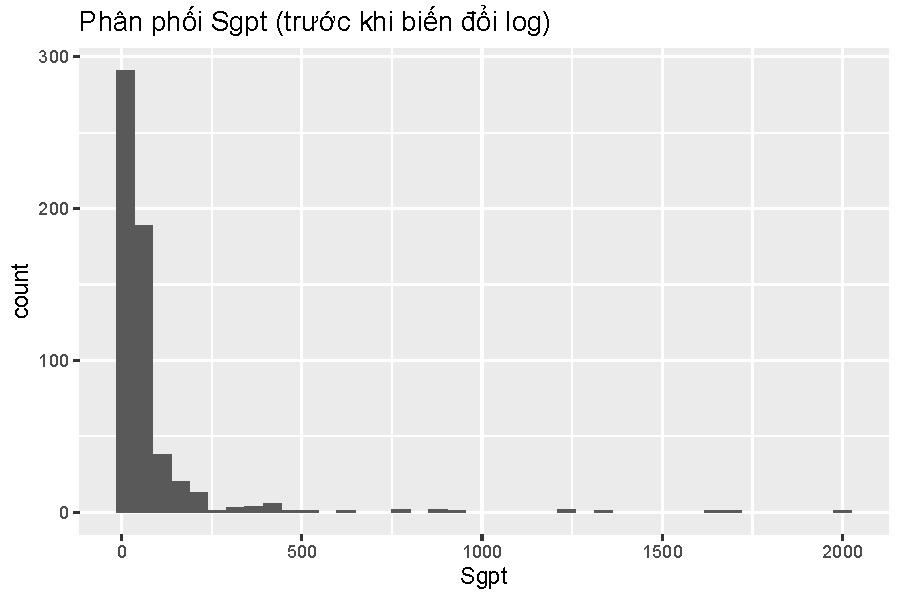
\includegraphics[width=\maxwidth]{figure/eda-sgpt-1} 

}

\caption[Phân phối Sgpt trước khi biến đổi log]{Phân phối Sgpt trước khi biến đổi log}\label{fig:eda-sgpt}
\end{figure}

\end{knitrout}

\subsection{Feature engineering}

Các biến TB, DB, Alkphos, Sgpt, Sgot thường lệch phải mạnh (outlier là các
ca bệnh nặng) --- biến đổi log giúp mô hình tuyến tính (logistic regression)
hoạt động ổn định hơn.

\begin{knitrout}\scriptsize
\definecolor{shadecolor}{rgb}{0.969, 0.969, 0.969}\color{fgcolor}\begin{kframe}
\begin{alltt}
\hldef{df} \hlkwb{<-} \hldef{df} \hlopt{%>%}
  \hlkwd{mutate}\hldef{(}
    \hlkwc{log_TB}      \hldef{=} \hlkwd{log1p}\hldef{(TB),}
    \hlkwc{log_DB}      \hldef{=} \hlkwd{log1p}\hldef{(DB),}
    \hlkwc{log_Alkphos} \hldef{=} \hlkwd{log1p}\hldef{(Alkphos),}
    \hlkwc{log_Sgpt}    \hldef{=} \hlkwd{log1p}\hldef{(Sgpt),}
    \hlkwc{log_Sgot}    \hldef{=} \hlkwd{log1p}\hldef{(Sgot)}
  \hldef{)}

\hldef{model_formula} \hlkwb{<-} \hldef{Selector} \hlopt{~} \hldef{Age} \hlopt{+} \hldef{Gender} \hlopt{+} \hldef{log_TB} \hlopt{+} \hldef{log_DB} \hlopt{+} \hldef{log_Alkphos} \hlopt{+}
  \hldef{log_Sgpt} \hlopt{+} \hldef{log_Sgot} \hlopt{+} \hldef{TP} \hlopt{+} \hldef{ALB} \hlopt{+} \hldef{AG_Ratio}
\end{alltt}
\end{kframe}
\end{knitrout}

% Viết ở đây: giải thích lý do log-transform, và có thể kiểm tra
% multicollinearity giữa TB-DB, Sgpt-Sgot (thường tương quan rất cao trong
% ILPD) bằng cor() hoặc corrplot nếu muốn mở rộng.

\section{Xây dựng \& lựa chọn mô hình bằng K-fold Cross-Validation}

Đây là phần trung tâm của quy trình Data Science: thay vì chọn 1 thuật
toán rồi báo cáo kết quả trên 1 lần chia train/test, ta dùng 10-fold CV
lặp lại (repeated k-fold) làm "trọng tài" khách quan để so sánh nhiều
mô hình.

\subsection{Thiết lập k-fold CV dùng chung}

\begin{knitrout}\scriptsize
\definecolor{shadecolor}{rgb}{0.969, 0.969, 0.969}\color{fgcolor}\begin{kframe}
\begin{alltt}
\hldef{ctrl_cv} \hlkwb{<-} \hlkwd{trainControl}\hldef{(}\hlkwc{method} \hldef{=} \hlsng{"repeatedcv"}\hldef{,} \hlkwc{number} \hldef{=} \hlnum{10}\hldef{,} \hlkwc{repeats} \hldef{=} \hlnum{3}\hldef{,}
                         \hlkwc{classProbs} \hldef{=} \hlnum{TRUE}\hldef{,}
                         \hlkwc{summaryFunction} \hldef{= twoClassSummary,}
                         \hlkwc{savePredictions} \hldef{=} \hlsng{"final"}\hldef{)}
\end{alltt}
\end{kframe}
\end{knitrout}

\subsection{So sánh nhiều mô hình trên cùng một cấu hình CV}

\begin{knitrout}\scriptsize
\definecolor{shadecolor}{rgb}{0.969, 0.969, 0.969}\color{fgcolor}\begin{kframe}
\begin{alltt}
\hldef{model_glm} \hlkwb{<-} \hlkwd{train}\hldef{(model_formula,} \hlkwc{data} \hldef{= df,} \hlkwc{method} \hldef{=} \hlsng{"glm"}\hldef{,} \hlkwc{family} \hldef{=} \hlsng{"binomial"}\hldef{,}
                    \hlkwc{trControl} \hldef{= ctrl_cv,} \hlkwc{metric} \hldef{=} \hlsng{"ROC"}\hldef{)}

\hldef{model_tree} \hlkwb{<-} \hlkwd{train}\hldef{(model_formula,} \hlkwc{data} \hldef{= df,} \hlkwc{method} \hldef{=} \hlsng{"rpart"}\hldef{,}
                     \hlkwc{trControl} \hldef{= ctrl_cv,} \hlkwc{metric} \hldef{=} \hlsng{"ROC"}\hldef{,} \hlkwc{tuneLength} \hldef{=} \hlnum{10}\hldef{)}

\hldef{model_rf} \hlkwb{<-} \hlkwd{train}\hldef{(model_formula,} \hlkwc{data} \hldef{= df,} \hlkwc{method} \hldef{=} \hlsng{"rf"}\hldef{,}
                   \hlkwc{trControl} \hldef{= ctrl_cv,} \hlkwc{metric} \hldef{=} \hlsng{"ROC"}\hldef{,} \hlkwc{tuneLength} \hldef{=} \hlnum{5}\hldef{)}

\hldef{results} \hlkwb{<-} \hlkwd{resamples}\hldef{(}\hlkwd{list}\hldef{(}\hlkwc{Logistic} \hldef{= model_glm,} \hlkwc{Tree} \hldef{= model_tree,} \hlkwc{RandomForest} \hldef{= model_rf))}
\hlkwd{summary}\hldef{(results)}
\end{alltt}
\begin{verbatim}
## 
## Call:
## summary.resamples(object = results)
## 
## Models: Logistic, Tree, RandomForest 
## Number of resamples: 30 
## 
## ROC 
##                   Min.   1st Qu.    Median      Mean   3rd Qu.
## Logistic     0.6638655 0.7043793 0.7455763 0.7508238 0.7820122
## Tree         0.5007622 0.6057081 0.6600161 0.6548229 0.6980907
## RandomForest 0.5861345 0.7202296 0.7412251 0.7484770 0.7999014
##                   Max. NA's
## Logistic     0.9061625    0
## Tree         0.7522866    0
## RandomForest 0.8258929    0
## 
## Sens 
##                   Min.   1st Qu.    Median      Mean   3rd Qu.
## Logistic     0.8292683 0.8780488 0.9024390 0.8983159 0.9213124
## Tree         0.6585366 0.7560976 0.7804878 0.7799845 0.8095238
## RandomForest 0.7857143 0.8536585 0.8809524 0.8824816 0.9268293
##                   Max. NA's
## Logistic     0.9761905    0
## Tree         0.9047619    0
## RandomForest 0.9756098    0
## 
## Spec 
##                    Min.   1st Qu.    Median      Mean   3rd Qu.
## Logistic     0.06250000 0.1994485 0.2500000 0.2851716 0.3750000
## Tree         0.05882353 0.2500000 0.3750000 0.3557598 0.4705882
## RandomForest 0.05882353 0.2352941 0.2720588 0.2769608 0.3125000
##                   Max. NA's
## Logistic     0.4705882    0
## Tree         0.5882353    0
## RandomForest 0.4705882    0
\end{verbatim}
\end{kframe}
\end{knitrout}

\begin{knitrout}\scriptsize
\definecolor{shadecolor}{rgb}{0.969, 0.969, 0.969}\color{fgcolor}\begin{kframe}
\begin{alltt}
\hlkwd{bwplot}\hldef{(results,} \hlkwc{metric} \hldef{=} \hlsng{"ROC"}\hldef{)}
\end{alltt}
\end{kframe}\begin{figure}

{\centering 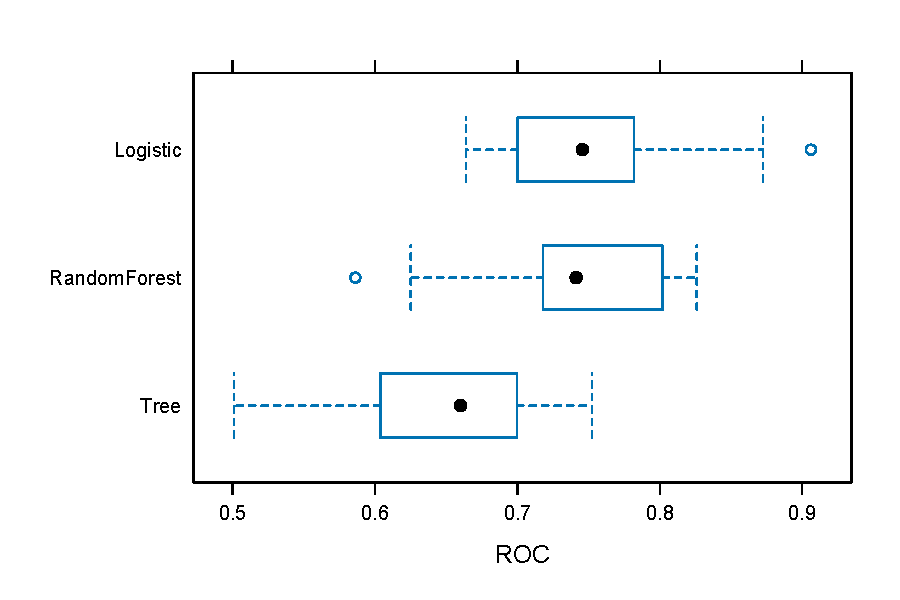
\includegraphics[width=\maxwidth]{figure/model-compare-plot-1} 

}

\caption[So sánh ROC giữa 3 mô hình qua k-fold CV]{So sánh ROC giữa 3 mô hình qua k-fold CV}\label{fig:model-compare-plot}
\end{figure}

\end{knitrout}

% Viết ở đây: mô hình nào có ROC/Sens/Spec trung bình cao nhất và ổn định
% nhất (độ lệch chuẩn thấp nhất qua các fold)? Đây là căn cứ để CHỌN mô hình
% cuối cùng - không phải chọn theo cảm tính mà theo bằng chứng từ CV.

\subsection{Mô hình được chọn: Logistic Regression}

Khác với Random Forest (tham số \texttt{mtry}) hay Decision Tree (tham số
\texttt{cp}), Logistic Regression cơ bản không có siêu tham số cần tinh
chỉnh qua k-fold CV --- đây cũng là một lý do được chọn làm mô hình cuối,
bên cạnh việc có hiệu năng cạnh tranh và dễ diễn giải hệ số hơn các mô
hình dạng cây.

\begin{knitrout}\scriptsize
\definecolor{shadecolor}{rgb}{0.969, 0.969, 0.969}\color{fgcolor}\begin{kframe}
\begin{alltt}
\hlkwd{summary}\hldef{(model_glm}\hlopt{$}\hldef{finalModel)}
\end{alltt}
\begin{verbatim}
## 
## Call:
## NULL
## 
## Coefficients:
##              Estimate Std. Error z value Pr(>|z|)    
## (Intercept)  8.496458   2.097030   4.052 5.09e-05 ***
## Age         -0.018335   0.006425  -2.854  0.00432 ** 
## GenderMale   0.092357   0.237019   0.390  0.69679    
## log_TB       0.346763   0.949722   0.365  0.71502    
## log_DB      -1.507719   1.108532  -1.360  0.17380    
## log_Alkphos -0.493192   0.277434  -1.778  0.07546 .  
## log_Sgpt    -0.780948   0.267349  -2.921  0.00349 ** 
## log_Sgot    -0.074994   0.232853  -0.322  0.74740    
## TP          -1.020444   0.388834  -2.624  0.00868 ** 
## ALB          1.925777   0.765132   2.517  0.01184 *  
## AG_Ratio    -2.169030   1.162884  -1.865  0.06215 .  
## ---
## Signif. codes:  0 '***' 0.001 '**' 0.01 '*' 0.05 '.' 0.1 ' ' 1
## 
## (Dispersion parameter for binomial family taken to be 1)
## 
##     Null deviance: 692.01  on 578  degrees of freedom
## Residual deviance: 567.82  on 568  degrees of freedom
## AIC: 589.82
## 
## Number of Fisher Scoring iterations: 6
\end{verbatim}
\end{kframe}
\end{knitrout}

\begin{knitrout}\scriptsize
\definecolor{shadecolor}{rgb}{0.969, 0.969, 0.969}\color{fgcolor}\begin{kframe}
\begin{alltt}
\hldef{final_model}      \hlkwb{<-} \hldef{model_glm}
\hldef{final_model_name} \hlkwb{<-} \hlsng{"Logistic Regression"}
\end{alltt}
\end{kframe}
\end{knitrout}

% Viết ở đây: dựa vào bảng so sánh CV ở trên, giải thích vì sao Logistic
% Regression được chọn (ROC/Accuracy tương đương hoặc tốt hơn, độ lệch chuẩn
% giữa các fold thấp, đồng thời dễ diễn giải hệ số hơn cho ứng dụng lâm sàng).

\section{Đánh giá độ tin cậy của mô hình cuối bằng Bootstrap}

K-fold CV đã giúp ta CHỌN được mô hình tốt nhất. Câu hỏi tiếp theo: hiệu
năng của mô hình này có đáng tin cậy không, hay chỉ là may rủi của 1 lần
lấy mẫu?

\subsection{Bootstrap khoảng tin cậy cho AUC của mô hình cuối}

\begin{knitrout}\scriptsize
\definecolor{shadecolor}{rgb}{0.969, 0.969, 0.969}\color{fgcolor}\begin{kframe}
\begin{alltt}
\hldef{boot_auc_fn} \hlkwb{<-} \hlkwa{function}\hldef{(}\hlkwc{data}\hldef{,} \hlkwc{indices}\hldef{) \{}
  \hldef{d} \hlkwb{<-} \hldef{data[indices, ]}
  \hldef{fit}  \hlkwb{<-} \hlkwd{glm}\hldef{(model_formula,} \hlkwc{data} \hldef{= d,} \hlkwc{family} \hldef{= binomial)}
  \hldef{pred} \hlkwb{<-} \hlkwd{predict}\hldef{(fit,} \hlkwc{type} \hldef{=} \hlsng{"response"}\hldef{)}
  \hlkwd{as.numeric}\hldef{(}\hlkwd{auc}\hldef{(}\hlkwd{roc}\hldef{(d}\hlopt{$}\hldef{Selector, pred,} \hlkwc{quiet} \hldef{=} \hlnum{TRUE}\hldef{)))}
\hldef{\}}

\hlcom{# Logistic regression fit nhanh nên có thể dùng R lớn hơn (1000)}
\hldef{boot_auc} \hlkwb{<-} \hlkwd{boot}\hldef{(df, boot_auc_fn,} \hlkwc{R} \hldef{=} \hlnum{1000}\hldef{)}
\hldef{boot_auc}
\end{alltt}
\begin{verbatim}
## 
## ORDINARY NONPARAMETRIC BOOTSTRAP
## 
## 
## Call:
## boot(data = df, statistic = boot_auc_fn, R = 1000)
## 
## 
## Bootstrap Statistics :
##      original     bias    std. error
## t1* 0.7713073 0.01361082  0.01949019
\end{verbatim}
\begin{alltt}
\hlkwd{boot.ci}\hldef{(boot_auc,} \hlkwc{type} \hldef{=} \hlsng{"perc"}\hldef{)}
\end{alltt}
\begin{verbatim}
## BOOTSTRAP CONFIDENCE INTERVAL CALCULATIONS
## Based on 1000 bootstrap replicates
## 
## CALL : 
## boot.ci(boot.out = boot_auc, type = "perc")
## 
## Intervals : 
## Level     Percentile     
## 95%   ( 0.7451,  0.8217 )  
## Calculations and Intervals on Original Scale
\end{verbatim}
\end{kframe}
\end{knitrout}

% Viết ở đây: khoảng tin cậy 95% của AUC cho biết mô hình dao động thế nào
% nếu áp dụng cho mẫu bệnh nhân khác - CI hẹp nghĩa là mô hình đáng tin cậy.

\subsection{Bootstrap đánh giá độ ổn định của hệ số hồi quy}

\begin{knitrout}\scriptsize
\definecolor{shadecolor}{rgb}{0.969, 0.969, 0.969}\color{fgcolor}\begin{kframe}
\begin{alltt}
\hldef{boot_coef_fn} \hlkwb{<-} \hlkwa{function}\hldef{(}\hlkwc{data}\hldef{,} \hlkwc{indices}\hldef{) \{}
  \hldef{d} \hlkwb{<-} \hldef{data[indices, ]}
  \hldef{fit} \hlkwb{<-} \hlkwd{glm}\hldef{(model_formula,} \hlkwc{data} \hldef{= d,} \hlkwc{family} \hldef{= binomial)}
  \hlkwd{coef}\hldef{(fit)}
\hldef{\}}

\hldef{boot_imp} \hlkwb{<-} \hlkwd{boot}\hldef{(df, boot_coef_fn,} \hlkwc{R} \hldef{=} \hlnum{1000}\hldef{)}

\hlcom{# Trung bình, độ lệch chuẩn và CI cho từng hệ số qua các lần bootstrap}
\hldef{imp_summary} \hlkwb{<-} \hlkwd{data.frame}\hldef{(}
  \hlkwc{Variable} \hldef{=} \hlkwd{names}\hldef{(boot_imp}\hlopt{$}\hldef{t0),}
  \hlkwc{Mean}     \hldef{=} \hlkwd{colMeans}\hldef{(boot_imp}\hlopt{$}\hldef{t),}
  \hlkwc{SD}       \hldef{=} \hlkwd{apply}\hldef{(boot_imp}\hlopt{$}\hldef{t,} \hlnum{2}\hldef{, sd)}
\hldef{)} \hlopt{%>%} \hlkwd{arrange}\hldef{(}\hlkwd{desc}\hldef{(}\hlkwd{abs}\hldef{(Mean)))}

\hldef{imp_summary}
\end{alltt}
\begin{verbatim}
##       Variable        Mean          SD
## 1  (Intercept)  9.01571968 2.319653456
## 2     AG_Ratio -2.43554261 1.421216633
## 3          ALB  2.11567470 0.932099228
## 4       log_DB -1.62682694 1.079687641
## 5           TP -1.11724969 0.471373885
## 6     log_Sgpt -0.80665572 0.279745633
## 7  log_Alkphos -0.51552378 0.293476230
## 8       log_TB  0.38391954 0.983155466
## 9   GenderMale  0.11528260 0.249394560
## 10    log_Sgot -0.08753967 0.239976120
## 11         Age -0.01868528 0.006440702
\end{verbatim}
\end{kframe}
\end{knitrout}

% Viết ở đây: biến nào có |Mean| lớn và SD nhỏ tương đối -> ảnh hưởng rõ và
% ổn định qua các mẫu; hệ số nào có CI (dùng boot.ci với index tương ứng)
% chứa giá trị 0 -> không có ý nghĩa thống kê ổn định, cẩn thận khi diễn
% giải trong thực tế lâm sàng.

\section{So sánh Bootstrap (.632) và K-fold trong đánh giá mô hình cuối}

Kiểm chứng chéo: nếu dùng .632 bootstrap thay vì k-fold để đánh giá lại
chính mô hình đã chọn, kết quả có nhất quán không?

\begin{knitrout}\scriptsize
\definecolor{shadecolor}{rgb}{0.969, 0.969, 0.969}\color{fgcolor}\begin{kframe}
\begin{alltt}
\hldef{ctrl_boot} \hlkwb{<-} \hlkwd{trainControl}\hldef{(}\hlkwc{method} \hldef{=} \hlsng{"boot632"}\hldef{,} \hlkwc{number} \hldef{=} \hlnum{200}\hldef{,}
                           \hlkwc{classProbs} \hldef{=} \hlnum{TRUE}\hldef{,} \hlkwc{summaryFunction} \hldef{= twoClassSummary)}

\hldef{model_boot} \hlkwb{<-} \hlkwd{train}\hldef{(model_formula,} \hlkwc{data} \hldef{= df,} \hlkwc{method} \hldef{=} \hlsng{"glm"}\hldef{,} \hlkwc{family} \hldef{=} \hlsng{"binomial"}\hldef{,}
                     \hlkwc{trControl} \hldef{= ctrl_boot,} \hlkwc{metric} \hldef{=} \hlsng{"ROC"}\hldef{)}

\hldef{model_boot}
\end{alltt}
\begin{verbatim}
## Generalized Linear Model 
## 
## 579 samples
##  10 predictor
##   2 classes: 'Disease', 'NoDisease' 
## 
## No pre-processing
## Resampling: Bootstrapped (200 reps) 
## Summary of sample sizes: 579, 579, 579, 579, 579, 579, ... 
## Resampling results:
## 
##   ROC        Sens       Spec     
##   0.7573377  0.8955657  0.2995401
\end{verbatim}
\begin{alltt}
\hlkwd{data.frame}\hldef{(}
  \hlkwc{Method} \hldef{=} \hlkwd{c}\hldef{(}\hlsng{"10-fold CV (x3 repeats)"}\hldef{,} \hlsng{".632 Bootstrap"}\hldef{),}
  \hlkwc{ROC}    \hldef{=} \hlkwd{c}\hldef{(model_glm}\hlopt{$}\hldef{results}\hlopt{$}\hldef{ROC, model_boot}\hlopt{$}\hldef{results}\hlopt{$}\hldef{ROC)}
\hldef{)}
\end{alltt}
\begin{verbatim}
##                    Method       ROC
## 1 10-fold CV (x3 repeats) 0.7508238
## 2          .632 Bootstrap 0.7573377
\end{verbatim}
\end{kframe}
\end{knitrout}

% Viết ở đây: 2 phương pháp cho kết quả gần nhau hay khác biệt? Nếu khác
% biệt đáng kể, giải thích bằng bias-variance tradeoff đã nêu ở phần lý
% thuyết. Đây là phần thể hiện rõ nhất bạn hiểu bản chất khác nhau của 2
% phương pháp, không chỉ biết cách gọi hàm.

\section{Kết luận}

% Viết ở đây:
% - Mô hình nào được chọn và vì sao (căn cứ từ k-fold CV)
% - Mô hình đó đáng tin cậy đến mức nào (căn cứ từ Bootstrap)
% - Biến sinh hóa nào quan trọng nhất và ổn định nhất trong dự đoán bệnh gan
% - Hạn chế: cỡ mẫu, mất cân bằng lớp, dữ liệu từ 1 vùng địa lý (Andhra Pradesh)
% - Hướng mở rộng nếu có (thêm mô hình, thêm dữ liệu, external validation)

\section{Tài liệu tham khảo}

Ramana, B. \& Venkateswarlu, N. (2022). ILPD (Indian Liver Patient Dataset)
[Dataset]. UCI Machine Learning Repository.
\url{https://doi.org/10.24432/C5D02C}

\end{document}
